
%\documentclass[xcolor=pdftex,dvipsnames,table]{beamer}
\documentclass[xcolor=pdftex,dvipsnames,table]{beamer}

\usetheme{Amsterdam}

\usefonttheme[onlymath]{serif}
\setbeamertemplate{navigation symbols}{}
\setbeamertemplate{footline}[frame number]

%\usepackage{paralist}
%\usepackage{enumerate}

\usepackage{colortbl}
\usepackage{lmodern}
\usepackage{comment}
\usepackage{natbib}
\usepackage{graphicx}
\usepackage{pbox}
\usepackage{pifont}
\usepackage{alltt}
\usepackage{verbatim}
\usepackage{multirow}
\usepackage{xspace}
\usepackage{cases}
\usepackage{geometry}
\usepackage{verbatim}
\usepackage{tikz}
\usepackage{pgf}
\usetikzlibrary{arrows,automata,positioning}
%\usepackage[absolute,overlay]{textpos}
\usepackage[normalem]{ulem}
\usepackage{tikz-qtree}
\usepackage{pbox}
\usepackage{amsopn}
%\usepackage{enumitem}
%\usepackage{ragged2e}
%\usepackage{pifont}

%\usepackage[all]{xy}

\usepackage{latexsym}
\usepackage{amsmath}
\usepackage{amssymb}
\usepackage{xfrac}

\usepackage{notation}
\usepackage{variables}
\usepackage{drawing}
%\usepackage{xparse}
%\usepackage{tikz}
%\usetikzlibrary{calc}
\usepackage{changepage}

\newcounter{savedenum}
\newcommand*{\saveenum}{\setcounter{savedenum}{\theenumi}}
\newcommand*{\resume}{\setcounter{enumi}{\thesavedenum}}

% declares a document
\begin{document}



	%\title{Employee's social media use}
	%\title{Social media use by employees}
	\title{Decoding for SMT}
	%\subtitle{for unsupervised language learning}

	\author{Wilker Aziz}
	\institute[UvA]{
		%\inst{1}
		Universiteit van Amsterdam\\
		\texttt{w.aziz@uva.nl}
	}

	\date{\today}
	
	% Title page
	{\setbeamertemplate{footline}{}
	\begin{frame}[plain]
		\titlepage
	\end{frame}
	}

	\frame{
	\frametitle{Decoding for SMT}
	
	\pause 
	We will be reasoning \\ \pause
	\begin{center}
		making decisions
	\end{center}
	
	\pause
	
	~ about solutions \\ \pause
	\begin{center}
		structures (translations)
	\end{center}
	
	\pause
	
	~ under a statistical model \\ \pause
	\begin{center}
		a function / a partial ordering
	\end{center}
	
	
}

\frame{
	\frametitle{Keywords}
	
	We need to better characterise 
	
	\begin{enumerate}
		\item<2-> space of solutions \\
		\textcolor{blue}{get to know the terrain}
		\item<3-> statistical model \\
		\textcolor{blue}{how to assess the importance of things}
		\item<4-> decision rules \\
		\textcolor{blue}{know what you want}
	\end{enumerate}
	
	
}

\frame{
	\frametitle{Terrain}
	
	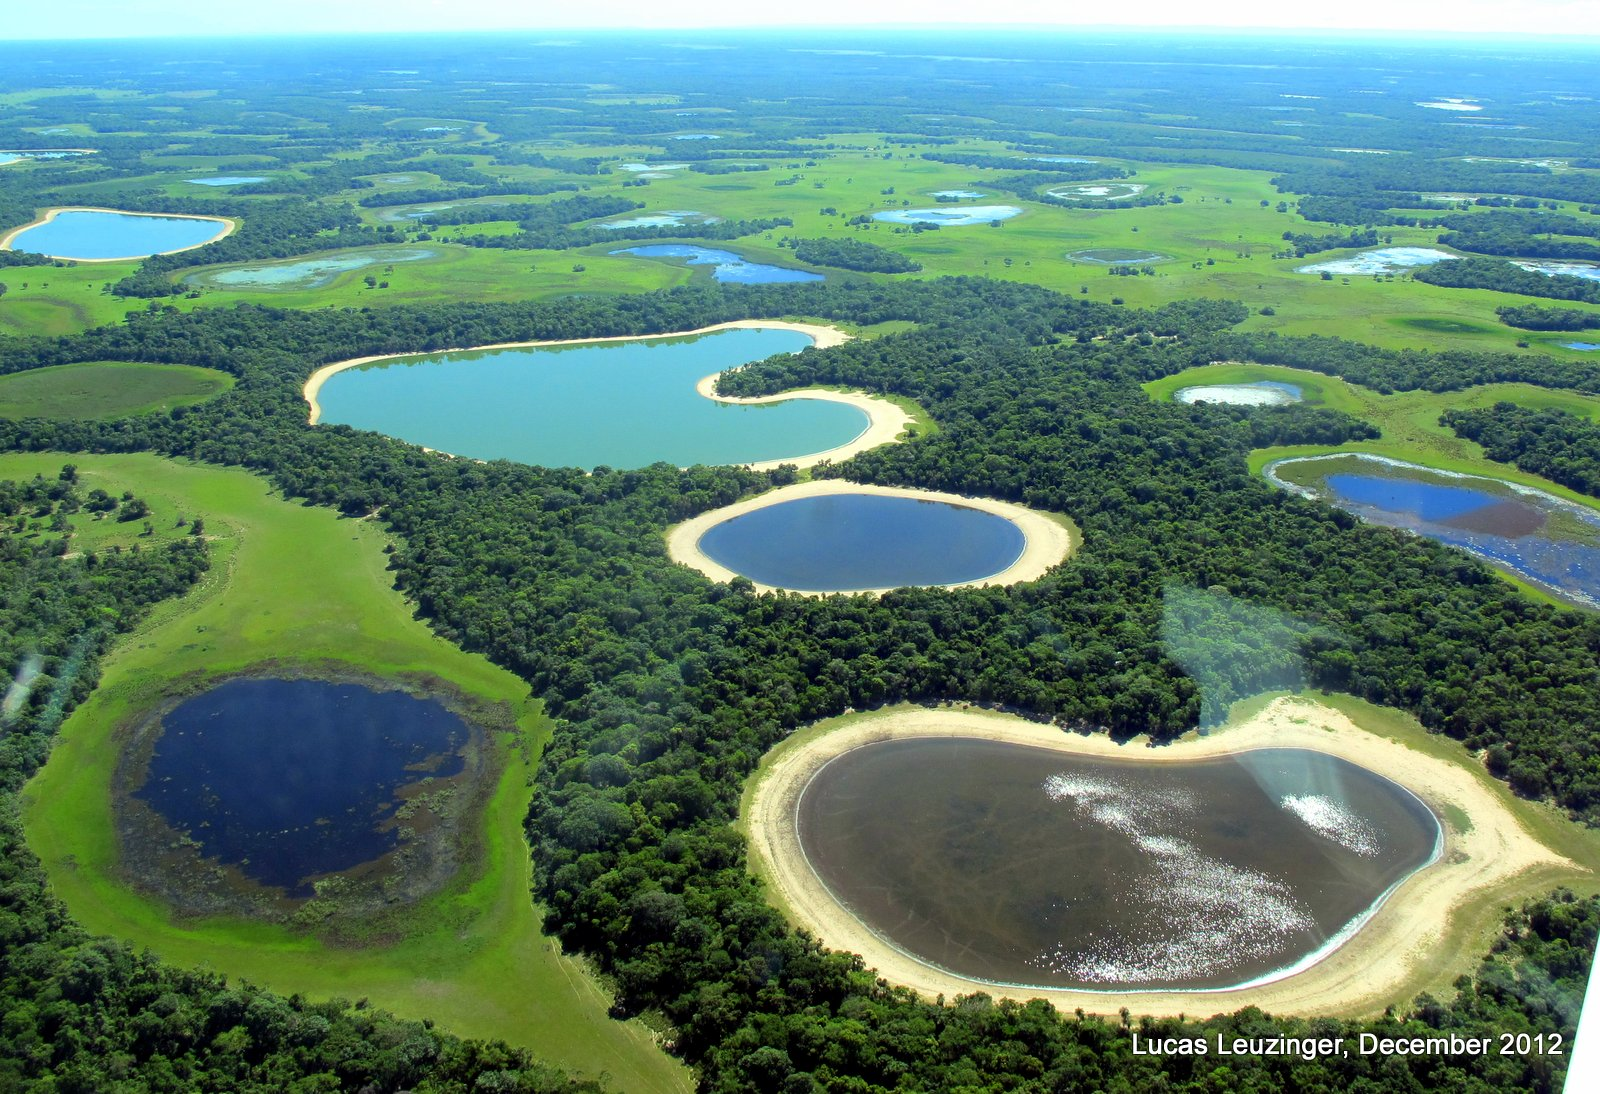
\includegraphics[scale=0.4]{img/pantanal} \pause
	
	not everywhere is a good place to stand
}

\frame{
	\frametitle{The importance (or cost) of things}
	
		
		\only<1>{
	
		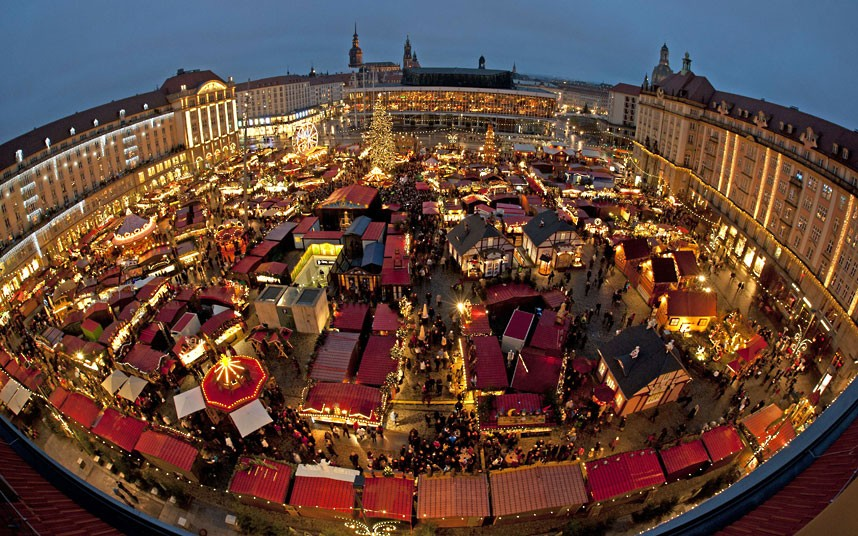
\includegraphics[scale=0.3]{img/demarket} 
		
		German xmas market
		
		}

		\only<2>{
		
		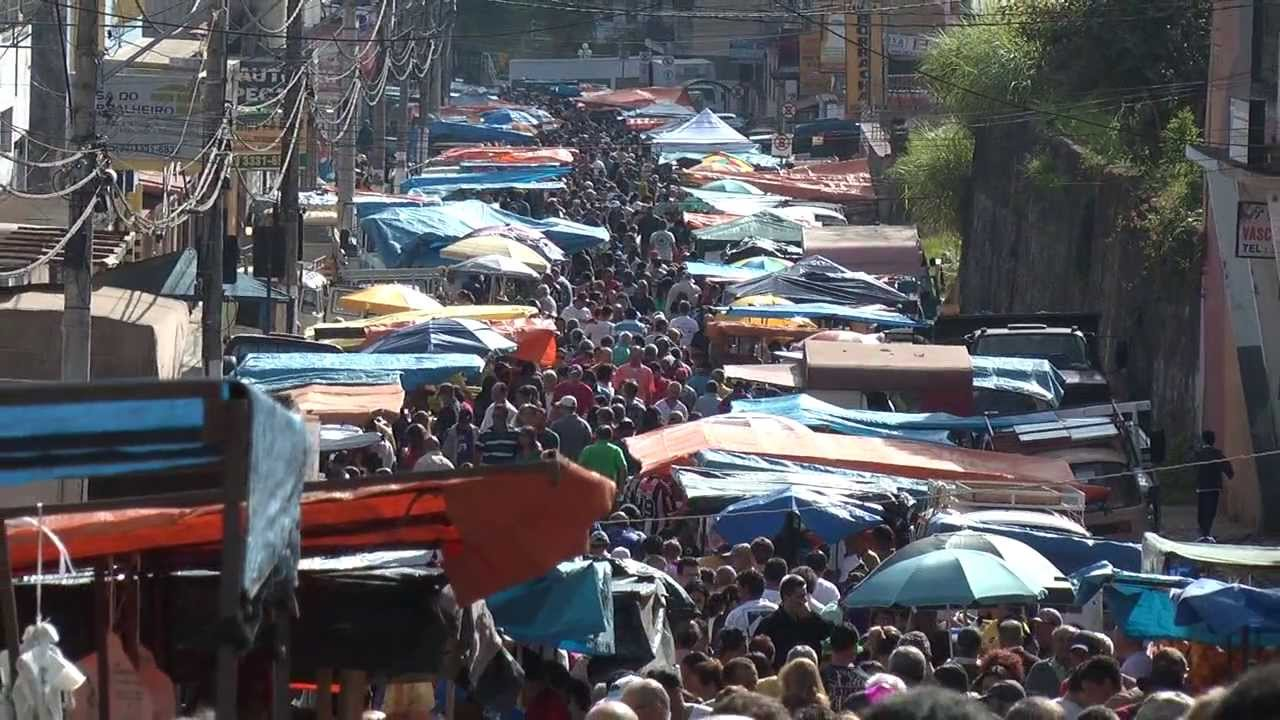
\includegraphics[scale=0.2]{img/brmarket}
		
		Brazilian street market
		
		}
		\only<3-6>{
		
			German xmas market
			\begin{columns}
				\begin{column}{0.4\textwidth}
					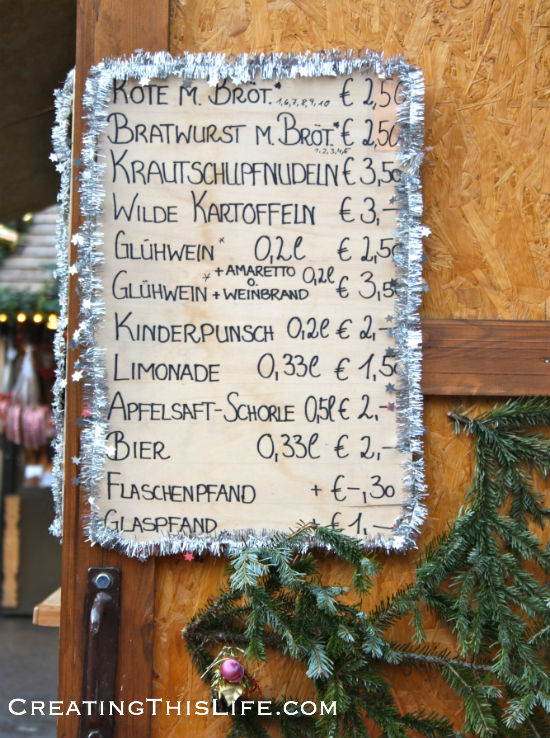
\includegraphics[scale=0.2]{img/demenu}
				\end{column}
				\begin{column}{0.45\textwidth}
					Price of product depends on
					\begin{itemize}
						\item<4-> the product
						\item<5-> brand
						\item<6-> quality of service
					\end{itemize}
				\end{column}
			\end{columns}
		}

		\only<7->{
		
			Brazilian street market
			\begin{columns}
				\begin{column}{0.4\textwidth}
					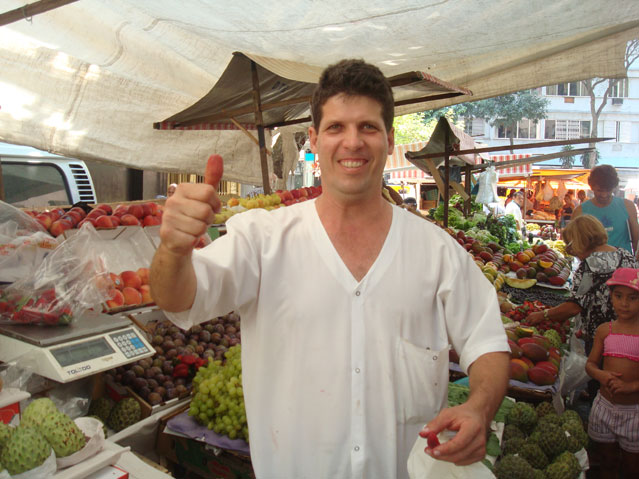
\includegraphics[scale=0.2]{img/feirante}
				\end{column}
				\begin{column}{0.45\textwidth}
					Price of product depends on
					\begin{itemize}
						\item the product
						\item brand
						\item quality of service
						\item<8-> seller's mood
						\item<9-> your look
						\item<10-> products you acquired from other stalls
						\item<11-> from whom you bought those
					\end{itemize}
				\end{column}
			\end{columns}
		}

}

\frame{
	\frametitle{Know what you want}
	
	\only<1>{
		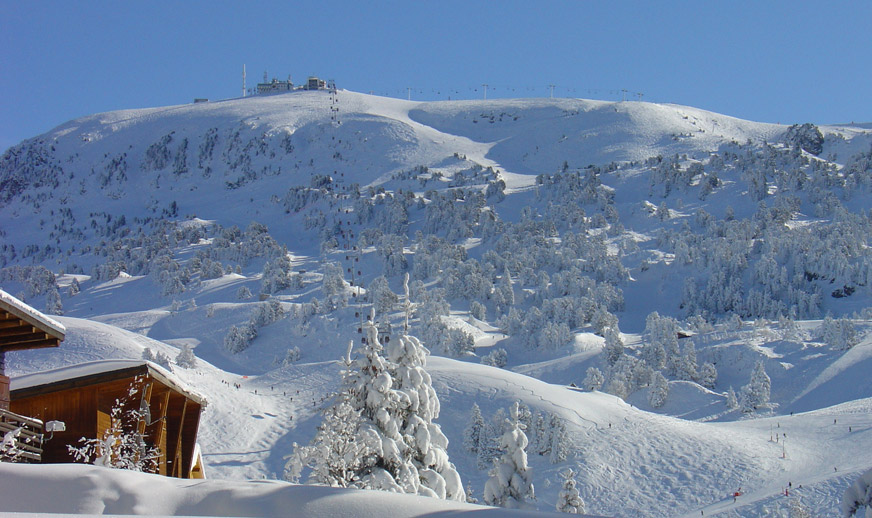
\includegraphics[scale=0.3]{img/station}
		
		what do you think when you see this picture?
	}
	\only<2>{
		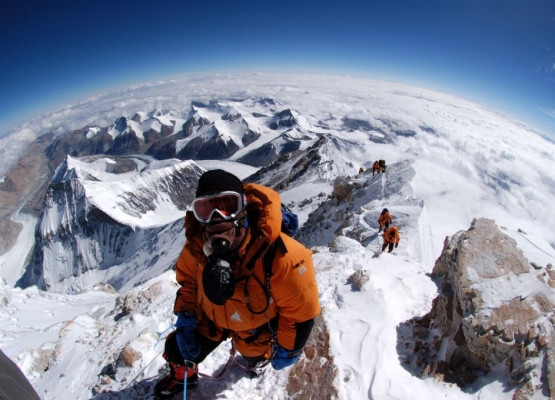
\includegraphics[scale=0.4]{img/top}
		
		make a selfie (and lose a couple of fingers in the process)?
	}
	\only<3>{
		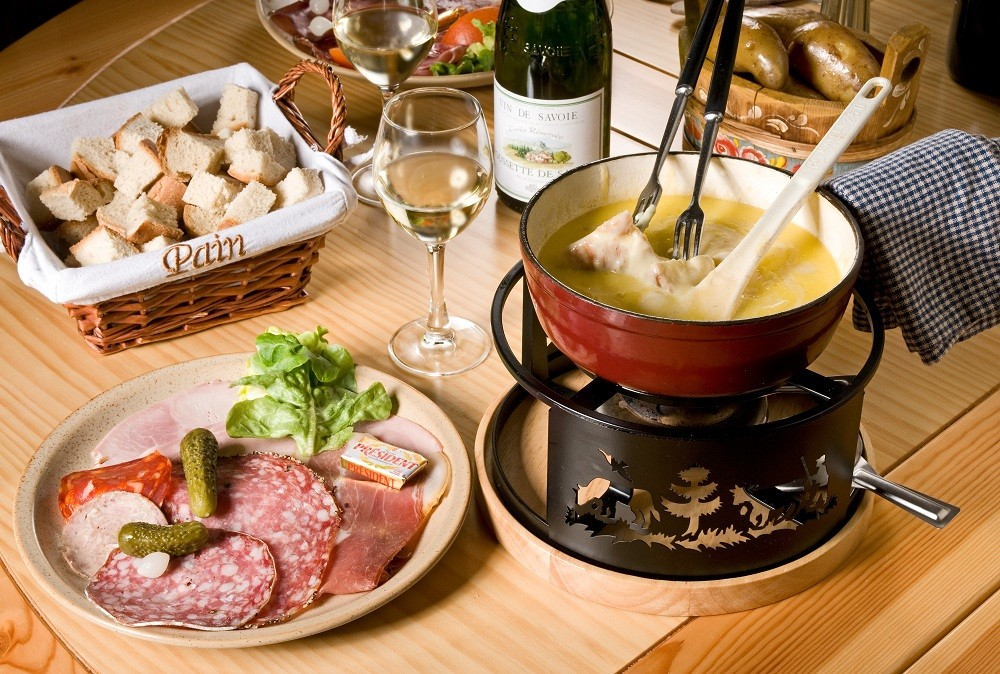
\includegraphics[scale=0.25]{img/dinner}
		
		French goodies in a cozy chalet?
	}
}



	% Table of contents	
	%\frame[allowframebreaks]{
	{\setbeamertemplate{footline}{}
	\begin{frame}
		\frametitle{Content}
		\tableofcontents
	\end{frame}
	}



	% trick to start counting from the table of contents
	\setcounter{framenumber}{0}


	% SLIDES
	\section{Space of translations}

\frame{
	\frametitle{Model of translational equivalences}
	
	Describes the process of generating translations of a given input
	\begin{itemize}
		\item constrains and characterises \\
		the set of possible translation derivations
	\end{itemize}
	
	\pause
	
	\begin{block}{Phrase-based MT}
	we observe an input, segment it into phrases, permute the phrases into  target language word-order, and finally, translate segments independently
	\end{block}
	
	\pause

	\begin{block}{Hierarchical MT}
	we parse the input with a CFG, then translate (using synchronous rules) each and every edge independently
	\end{block}
	
}

\frame{
	\frametitle{CFGs and FSAs}
	
	Compactly represent the set of translations
	\begin{itemize}
		\item keep the representation cost a tractable (polynomial) function of the input length
	\end{itemize}
	
	~
	
	
	Phrase-based MT $O(n^2 2^d)$
	
	~
	
	Hierarchical MT $O(n^3)$
}

\frame{
	\frametitle{Independence assumptions}
	
	Translation rules (flat or CFG) are applied independently
	
	\only<2>{
	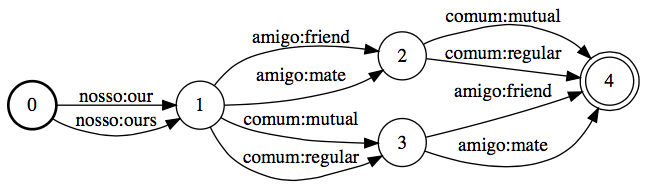
\includegraphics[scale=0.4]{img/fsa}
	}
	\only<3>{
	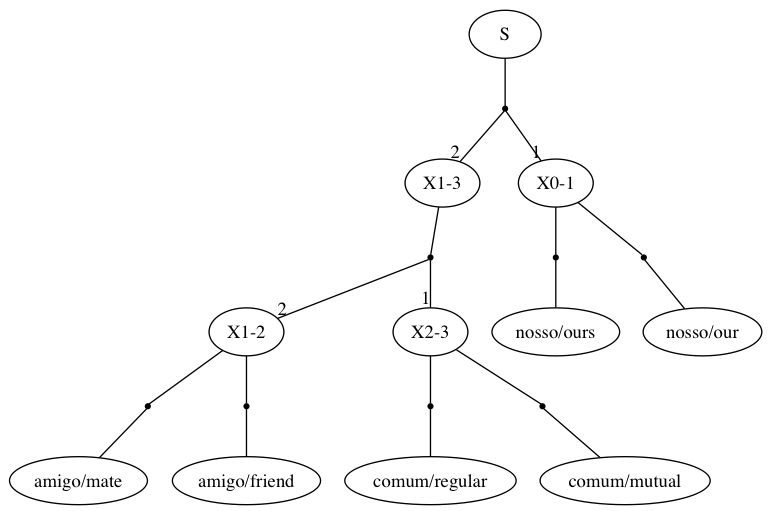
\includegraphics[scale=0.4]{img/cfg}
	}
	
}


	\section{Formal devices}

\frame{
	\frametitle{Directed B-hypergraphs}
	
	A hypergraph $\angbrack{V, E}$ consists of
	\begin{itemize}
		\item a set of nodes $V$
		\item a set of edges $E$
		\item an edge $e$ has 
		\begin{itemize}
			\item a head node $\head(e) \in V$ 
			\item a tail $\tail(e) \in V^*$ (sequence of nodes)
		\end{itemize}
		%\item $BS(v)$ is the set of incoming edges to $v$
	\end{itemize}
	
	\pause
	
	\begin{footnotesize}
	\begin{columns}
	\begin{column}{0.5\textwidth}
	CFGs
	\begin{itemize}%[noitemsep,nolistsep]
		\item nonterminal \ra node
		\item terminal \ra terminal node 
		\item rule \ra edge
		\item LHS \ra head
		\item RHS \ra tail
	\end{itemize}
	\end{column}
	\pause
	\begin{column}{0.5\textwidth}
	FSAs
	\begin{itemize}%[noitemsep,nolistsep]
		\item state \ra node
		\item symbol \ra terminal node
		\item transition \ra edge
		\item origin \ra tail node
		\item destination \ra head
	\end{itemize}
	\end{column}
	
	\end{columns}
	\end{footnotesize}
		
	
}

\frame{
	\frametitle{A forest as a hypergraph}
	
	\begin{center}
	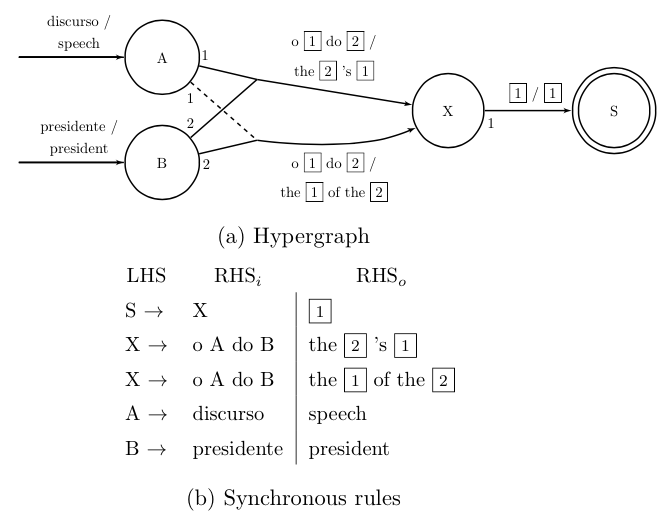
\includegraphics[scale=0.4]{img/hg}
	\end{center}
	
}

\frame{
	\frametitle{Weighted sets}
	
	A weighted set $\angbrack{\mDD, \omega}$ consists of 
	\begin{itemize}
		\item a set of structures (e.g. hyperpaths/derivations)
		\item a function $w : \mDD \ra \mathcal{K}$
	\end{itemize}
	
	~
	
	Let us focus on weighted sets whose weight functions factorise
				$$w(\mdd) = \bigotimes_{e \in \mdd} w(e)$$ 
				
	~
	
	Often the structure is just a means to an end (the yield)
			$$w(\myy) = \bigoplus_{\mdd \in \mDD_\myy} w(\mdd)$$ 
	
}

\frame{
	\frametitle{Semirings}
	
	An algebraic structure $\mathcal{K} = \angbrack{\mathbb{K}, \oplus, \otimes, \bar{0}, \bar{1}}$ \pause
	\begin{itemize}
		\item $\mathbb K$ is a set (e.g. $\mathbb N, \mathbb R, \{0, 1\}$) \pause
		\item $\oplus$ and $\otimes$ are binary operators \pause
		\item $\oplus$ is commutative and has identity $\bar{0}$\\ 
		$a \oplus b = b \oplus a$ and $\bar{0} \oplus a = a \oplus \bar{0} = a$ \pause
		\item $\otimes$ is associative and has identity $\bar{1}$\\
		$(a \otimes b) \otimes c = a \otimes (b \otimes c)$ and $\bar{1} \otimes a = a \otimes{1} = a$ \pause
		\item $\otimes$ left distributes over $\oplus$\\
		$a \otimes (b \oplus c) = (a \otimes b) \oplus (a \otimes c)$ \pause
		\item $\bar{0}$ is the $\otimes$-annihilator \\
		$\bar{0} \otimes a = a \otimes \bar{0} = \bar{0}$
	\end{itemize}
}

\frame{
	\frametitle{Examples of semirings}
	
	
	\begin{center}
	\begin{tabular}{l | c | c | c | c | c}
	Name      & $\mathbb K$ & $\oplus$& $\otimes$& $\bar{0}$ & $\bar{1}$\\ \hline \hline
	\textsc{Binary}    & $\{0, 1\}$  & $\vee $ & $\wedge$ & $0$ & $1$ \\
	\textsc{Counting}  & $\mathbb N$ & $+$     & $\times$ & $0$ & $1$ \\
	\textsc{Prob}      & $[0, 1] \subset \mathbb R$ & $+$     & $\times$ & $0$ & $1$ \\
	\textsc{LogProb}   & $\mathbb R \cup \{-\infty\}$ & $\oplus_{\log}$ & $+$ & $-\infty$ & $0$\\
	\textsc{Viterbi}   & $\mathbb R \cup \{-\infty\}$ & $\max$ & $+$  & $-\infty$ & $0$\\
	\end{tabular}
	\end{center}
	
	~
	
	where $a \oplus_{\log} b = \log(\exp(a) + \exp(b))$
}
	\section{Linear models}

\frame{
	\frametitle{Linear models}
	
	$$f(\mdd) = \mww^\top \bPhi(\mdd)$$
	
	where
	\begin{itemize}
		\item $\mww \in \Reals^m$ 
		\item $\bPhi(\mdd) = \angbrack{\Phi_1(\mdd), \ldots, \Phi_m(\mdd)}$
		\item $\Phi_i(\mdd) \in \Reals$ is a feature function
		\item $w_i$ is the relative contribution of the $i$th feature
	\end{itemize}
}

\frame{
	\frametitle{Linear models and independence assumptions}
	
	\begin{align}
		f(\mdd) 
		 &= \mww^\top \bPhi(\mdd) \\
		 &= \sum_{i=1}^m w_i \Phi_i(\mdd)  \\ 
		 &= \sum_{i=1}^m w_i  \prod_{e \in \mdd} \phi_i(e)   \\ 
		 &= \prod_{e \in \mdd} \sum_{i=1}^m w_i \phi_i(e)  \\ 
		 &= \prod_{e \in \mdd} \mww^\top \bphi(e)
	\end{align}
	
	Assumption
	\begin{itemize}
		\item $\Phi_i(\mdd)$ factorises over edges\\
		$\phi_i(e)$ is a local feature function
	\end{itemize}
}

\frame{
	\frametitle{Linear models and CFGs}
	
	Linear models can be expressed through hypergraphs using an appropriate semiring
	
}

\section{Decision rules}

\frame{
	\frametitle{Decision rules}

	Best translation (MAP)
	$$\myy\ustar = \argmax_{\myy} \sum_{d \in \mDD_\myy} f(\mdd)$$
	
	~ \pause
	
	Best derivation (Viterbi)
	$$\myy\ustar \approx \yield\left\{\argmax_{\mdd} f(\mdd)\right\}$$
	\begin{itemize}
		\item less disambiguation power
		\item \textsc{Viterbi} semiring
	\end{itemize}
}

\frame{
	\frametitle{Other decision rules?}
	
	Minimum Bayes risk (MBR)
	$$\myy\ustar = \argmin_{\myy'} \expec{L(\myy', \myy)}{p(\myy)}$$
	
	\begin{itemize}
		\item requires the underlying model to have a probabilistic interpretation
		\item can be estimated through sampling
	\end{itemize}
	
	\pause
	
	Log-linear models
	$$p(\mdd) = \frac{\exp(f(\mdd))}{\sum_{\mdd'} \exp(f(\mdd'))} \propto \exp\left(\sum_{e \in \mdd} \mww^\top \bphi(e)\right) = \prod_{e \in \mdd} \exp(\mww^\top \bphi(e))$$
	\hfill \textsc{LogProb} semiring
	
	
}
	\section{Decoding}
\subsection{Complexity}
\frame{
        \frametitle{Decoding}

        Disambiguation problem
        \begin{align*}
                \hat{E} 
                &= \argmax_E P(E)P(F|E) \\
                &= \argmax_E P(E) \sum_A P(F,A|E)
        \end{align*}
        {\small \hfill NP-complete \citep{Simaan:2002:complexity}}

        \pause

        ~

        Viterbi approximation
        \begin{align*}
                \hat{E} 
                &\approx \argmax_{E, A} P(E) P(F,A|E)\\
        \end{align*}

}

\frame{
	\frametitle{Viterbi decoding}
	The alignment space (or space of \emph{derivations})
	\begin{itemize}
		\item $O(2^n)$ segmentations\\
		\item $O(n!)$ permutations\\
		\item $O(t^n)$ substitutions\\
	\end{itemize}
	\pause
	~
	
	Packed representation using finite-state transducers
	$$O(n^2 \times \alert{2^n} \times t)$$
	\hfill NP-complete (TSP) \citep{Knight:1999:tsp,Zaslavskiy+2009:tsp} 
	
	
}

\frame{
	\frametitle{Complete model}
	
	\begin{align*}
		\alert{P(E)}P(F,S|E) 
		&= \alert{\prod_{j=1}^{|E|} \psi(e_j|e_{j - n + 1}^{j - 1})} \prod_{i=1}^{|S|} \textcolor{blue}{\phi(\bar{f}_i|\bar{e}_i)} \textcolor{Green}{\delta(\text{start}_i - \text{end}_{i-1} - 1)}
	\end{align*}

	Approximations:
	\begin{itemize}
		\item distortion limit $d$: $2^n \to 2^d$
		\item maximum phrase length $m$: $n^2 \to n \times m$
	\end{itemize}
	
	~

	\begin{itemize}

		\item alignment space $O(\textcolor{Green}{2^d} \times \textcolor{blue}{n \times m}\times t )$
		\item weighted derivations $O(\textcolor{Green}{2^d} \times \textcolor{blue}{n \times m} \times t \times \alert{|\Delta|^{k-1}})$ \\
		where $P(E)$ is a $k$-gram LM components over $\Delta^*$\\
		and $|\Delta| \propto t \times n$
	\end{itemize}

	\only<2->{
	\textbf<2->{This space is too large for exact inference}
	\begin{itemize}
		\item<3> pruning: beam search
	\end{itemize}
	}
	
}

\frame{
    \frametitle{Complexity}
	 \citep{Knight:1999:tsp}
	\begin{center}
       \only<1>{
                \includegraphics[width=0.7\textwidth]{"img/knight-tsp1"}
        }
        \only<2>{
                \includegraphics[width=0.5\textwidth]{"img/knight-tsp2"}
        }
	\end{center}
}

	
	\newcounter{finalframe}
	\setcounter{finalframe}{\value{framenumber}}
	
	
	{\setbeamertemplate{footline}{}
    \begin{frame}[plain]{Questions?}
    \end{frame}
  	}
	
	
	%
\frame[plain]{
	\frametitle{Earley intersection}
	
	\begin{footnotesize}
	\begin{align*}
	\textsc{Axioms} & \\
	& \drule{}{\itembrack{S' \ra \bullet S, q, q}}{q \in I} \\
	\textsc{Goal} & \\
	& \itembrack{S' \ra S \bullet, q, r} ~ q \in I \wedge r \in F\\
	\textsc{Scan} & \\
	& \drule{\itembrack{X \ra \alpha \bullet x \beta, q, s}}{\itembrack{X \ra \alpha x \bullet \beta}}{\angbrack{s, x, r} \in E}\\
	\textsc{Predict} & \\
	& \drule{\itembrack{X \ra \alpha \bullet Y \beta, q, r}}{\itembrack{Y \ra \bullet \gamma, r, r}}{Y \ra \gamma \in R} \\
	\textsc{Complete} & \\
	& \drule{\itembrack{X \ra \alpha \bullet Y \beta, q, s}\itembrack{Y \ra \gamma \bullet, s, r}}{\itembrack{X \ra \alpha Y_{s,r} \bullet \beta, q, r}}{X \neq S'} \\
	\textsc{Accept} & \\
	& \drule{\itembrack{S' \ra \bullet S, q, q}\itembrack{S \ra \gamma \bullet, q, r}}{\itembrack{S' \ra  S_{q,r} \bullet, q, r}}{r \in F} 
	\end{align*}
	\end{footnotesize}

	
}




	\frame[allowframebreaks]{ \frametitle{References}
        \bibliographystyle{plainnat}
        \bibliography{../bib}
	}

	

	% Trick to discount regular frames from the total of backup frames
	\setcounter{framenumber}{\value{finalframe}}
	
	
\end{document}
